\definecolor{mygreen}{rgb}{0,0.6,0}
\definecolor{mygray}{rgb}{0.5,0.5,0.5}
\definecolor{mymauve}{rgb}{0.58,0,0.82}

\lstset{ %
  backgroundcolor=\color{white},   % choose the background color; you must add \usepackage{color} or \usepackage{xcolor}
  basicstyle=\footnotesize,        % the size of the fonts that are used for the code
  breakatwhitespace=false,         % sets if automatic breaks should only happen at whitespace
  breaklines=true,                 % sets automatic line breaking
  captionpos=b,                    % sets the caption-position to bottom
  commentstyle=\color{mygreen},    % comment style
  deletekeywords={...},            % if you want to delete keywords from the given language
  %escapeinside={\%*}{*)},          % if you want to add LaTeX within your code
  %extendedchars=true,              % lets you use non-ASCII characters; for 8-bits encodings only, does not work with UTF-8
  %frame=single,	                   % adds a frame around the code
  keepspaces=true,                 % keeps spaces in text, useful for keeping indentation of code (possibly needs columns=flexible)
  keywordstyle=\color{blue},       % keyword style
  language=[ANSI]C,					% the language of the code
  %otherkeywords={*,...},           % if you want to add more keywords to the set
  numbers=left,                    % where to put the line-numbers; possible values are (none, left, right)
  numbersep=5pt,                   % how far the line-numbers are from the code
  numberstyle=\tiny\color{mygray}, % the style that is used for the line-numbers
  rulecolor=\color{black},         % if not set, the frame-color may be changed on line-breaks within not-black text (e.g. comments (green here))
  showspaces=false,                % show spaces everywhere adding particular underscores; it overrides 'showstringspaces'
  showstringspaces=false,          % underline spaces within strings only
  showtabs=false,                  % show tabs within strings adding particular underscores
  stepnumber=1,                    % the step between two line-numbers. If it's 1, each line will be numbered
  stringstyle=\color{mymauve},     % string literal style
  tabsize=2,	                   % sets default tabsize to 2 spaces
  title=\lstname,                   % show the filename of files included with \lstinputlisting; also try caption instead of title
  morecomment=[s]{/*}{*/}%
}



\chapter{Diseño e Implementación} % Main chapter title
\label{Chapter3} % Change X to a consecutive number; for referencing this chapter elsewhere, use \ref{ChapterX}
%----------------------------------------------------------------------------------------
%	SECTION 1
%----------------------------------------------------------------------------------------
Aquí se presenta el detalle del hardware planteado como un \enquote{poncho} sobre la EDU-CIAA, y la interfaz con los elementos de la planta. Luego se describe la estructura lógica del software con detalles del diseño sobre diagramas de interacción entre tareas, diagramas de capas y otras consideraciones relevantes del código.


\section{Análisis del Hardware}
\label{analisis_hardware}
El prototipo se implemento sobre una EDU-CIAA en conjunto con un hardware de adaptación de las interfaces. Para ello se utilizaron los proyectos de código abierto Kicad \citep{kicad} para la elaboración del poncho de la EDU-CIAA \citep{brengiponchos} que adapta las entradas y salidas de los conectores de expansión con los sensores y actuadores utilizados en la planta. 

\subsection{ Sensores y actuadores }

% Aca van todo lo referido a consideraciones importantes sobre los esquematicos.
%\subsubsection{Esquemáticos del prototipo final}

Para la adaptación de las interfaces con termocuplas y termistores se necesitaron circuitos de adaptación de señal. Para el primer caso se uso un circuito integrado compensador de juntura debido a la alinealidad en la respuesta de ese tipo de sensores. Para ello se eligió el MAX31855KASA+ \footnotemark como una solución simplificadora. 
También existen soluciones implementadas con amplificadores multietapas que son mas económicos pero que obligan a implementar la transducción de la señal en el microprocesador \citep{interOpamp}.\\
En la Figura \ref{fig:cirCompTermocupla} se observa una configuración típica de adaptación para termocupla.

\footnotetext{\url{bucar la url con la hoja de datos}} 

\begin{figure}[h!]
	\centering
	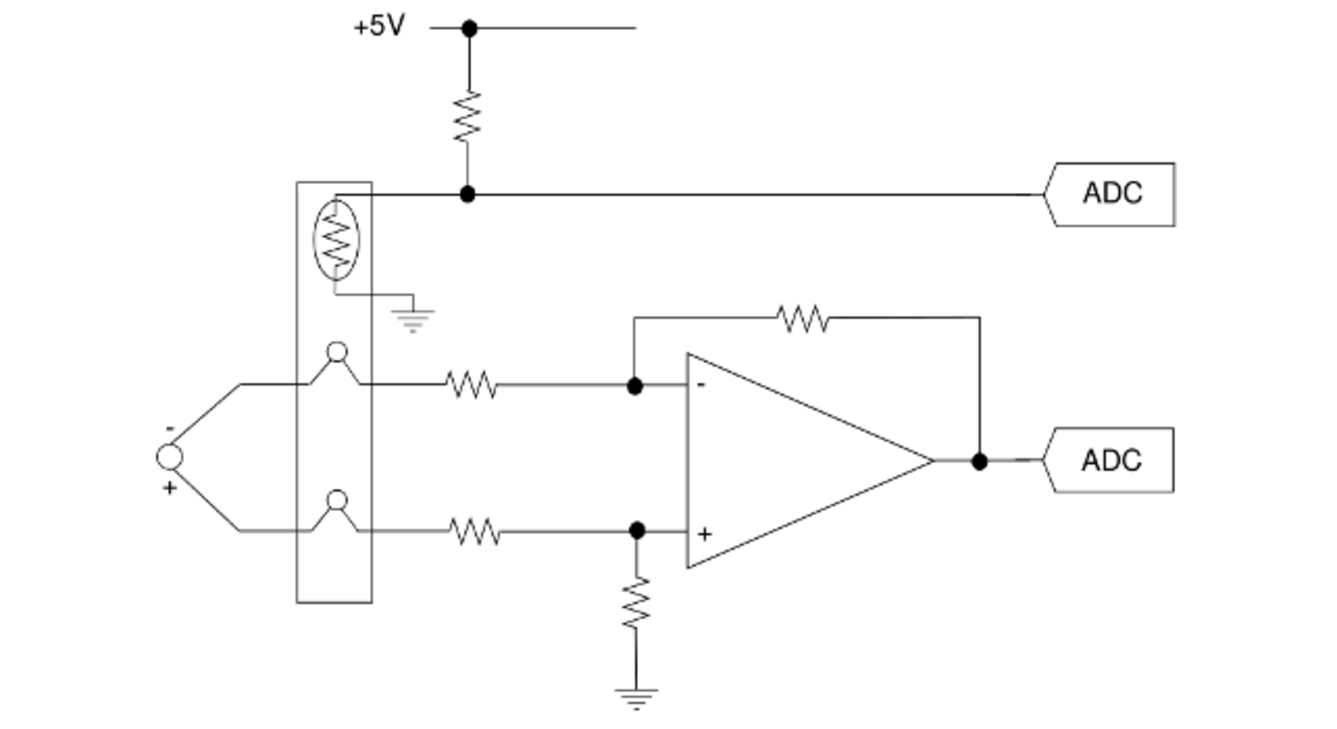
\includegraphics[width=.7\textwidth]{Figures/Cap_3/circuito_ampl_termocupla}
	\caption{Circuito simplificado de amplificación y compensación de termocuplas.}
	\label{fig:cirCompTermocupla}
\end{figure}

En el caso del termistor el circuito de adaptación es mas simple debido a que señal obtenida es prácticamente lineal y solamente es necesario amplificar a los niveles de trabajo de la entrada analógica del procesador. En la Figura \ref{fig:cirCompTermistor} se observa en tipo de circuito que se implementó.

\begin{figure}[h!]
	\centering
	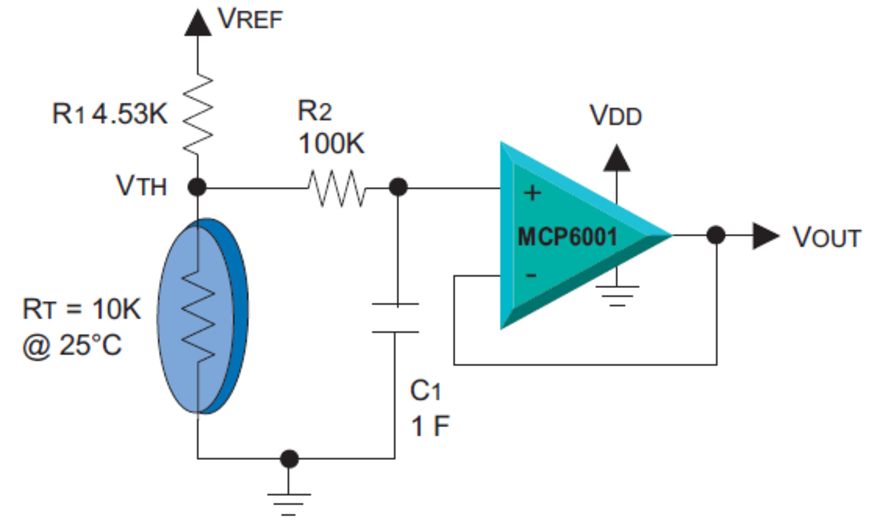
\includegraphics[width=.7\textwidth]{Figures/Cap_3/thermistor-conventional-circuit}
	\caption{Circuito simplificado de amplificación y compensación de termistores.}
	\label{fig:cirCompTermistor}
\end{figure}

En el caso de la medición de corriente y tension continua para las pruebas solo se consideraron sensores de baja potencia a fin de poder validar el comportamiento. Cabe aclarar que en linea de producción las fuentes de galvanizado son de muy alta potencia y la intensidad es leída actualmente con pinzas amperímetros AC/DC.
La medición de tension se toma en principio con un circuito aislado con foto-transistores para obtener mayor aislación de la fuente de corriente.
La medición de continuidad o salinidad del agua se resolvió implementarla con un circuito de terceros conectado a través de una de las entradas analógicas del prototipo. Las señales a medir son tensiones capacitivas entre dos varillas metálicas de muy bajo valor, la cuales se necesita acondicionar con operacionales de muy bajo piso de ruido o circuitos conversores analógicos digitales cerca del sensor.

Respecto a los actuadores se resolvió implementarlos con relés electromecánicos mas los circuitos de protección por sobre-picos de tension. Estos irán conectados a contactores que habilitan los distintos dispositivos como son: resistencias eléctricas, aireadores, alarmas, indicadores luminosos, etc.

\subsection{ Conexión al \enquote{poncho} diseñado }

En función de los periféricos que se acordaron utilizar en el prototipo, se diseñó un placa de expansión o poncho para utilizar con la EDU-CIAA a fin de tener un plataforma de prueba mas confiable. 

%\subsection{ Conexion de perifericos }
Según las configuraciones de la sección \ref{subsec:casos_de_uso} y en función de los puertos disponibles de la EDU-CIAA, se establecieron dos modos de conexión de sensores y actuadores. En la figuras \ref{fig:conectPerifericos1} y \ref{fig:conectPerifericos2} se observa como se corresponderían las conexiones a los periféricos del prototipo en función de los modos de uso. 

% Colocar diagrama de conexion
\begin{figure}[h!]
	\centering
	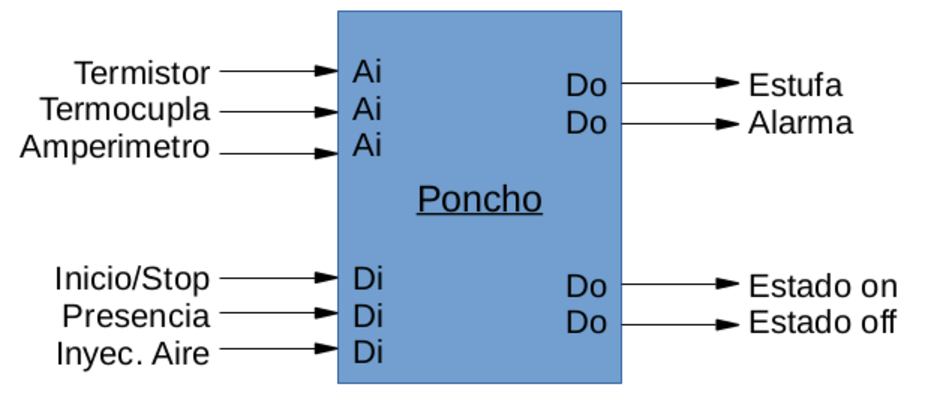
\includegraphics[width=.7\textwidth]{Figures/Cap_3/conexion_modo_1}
	\caption{Conexión en modo funcionamiento 1}
	\label{fig:conectPerifericos1}
\end{figure}

\begin{figure}[h!]
	\centering
	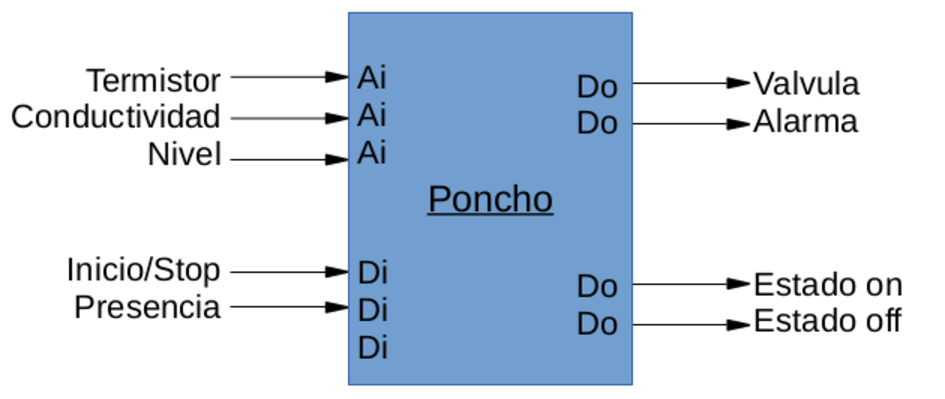
\includegraphics[width=.78\textwidth]{Figures/Cap_3/conexion_modo_2}
	\caption{Conexión en modo funcionamiento 2.}
	\label{fig:conectPerifericos2}
\end{figure}

Los puertos están preconfigurados y tienen asignaciones de pines predeterminadas, no obstante estos pueden modificarse desde la terminal al ingresar al modo de configuración.

En las figuras \ref{fig:renderPonchoTOP} y \ref{fig:renderPonchoBOT} se muestran las vistas del prototipo propuesto para desarrollar en el sistema piloto. 

\begin{figure}[h!]
	\centering
	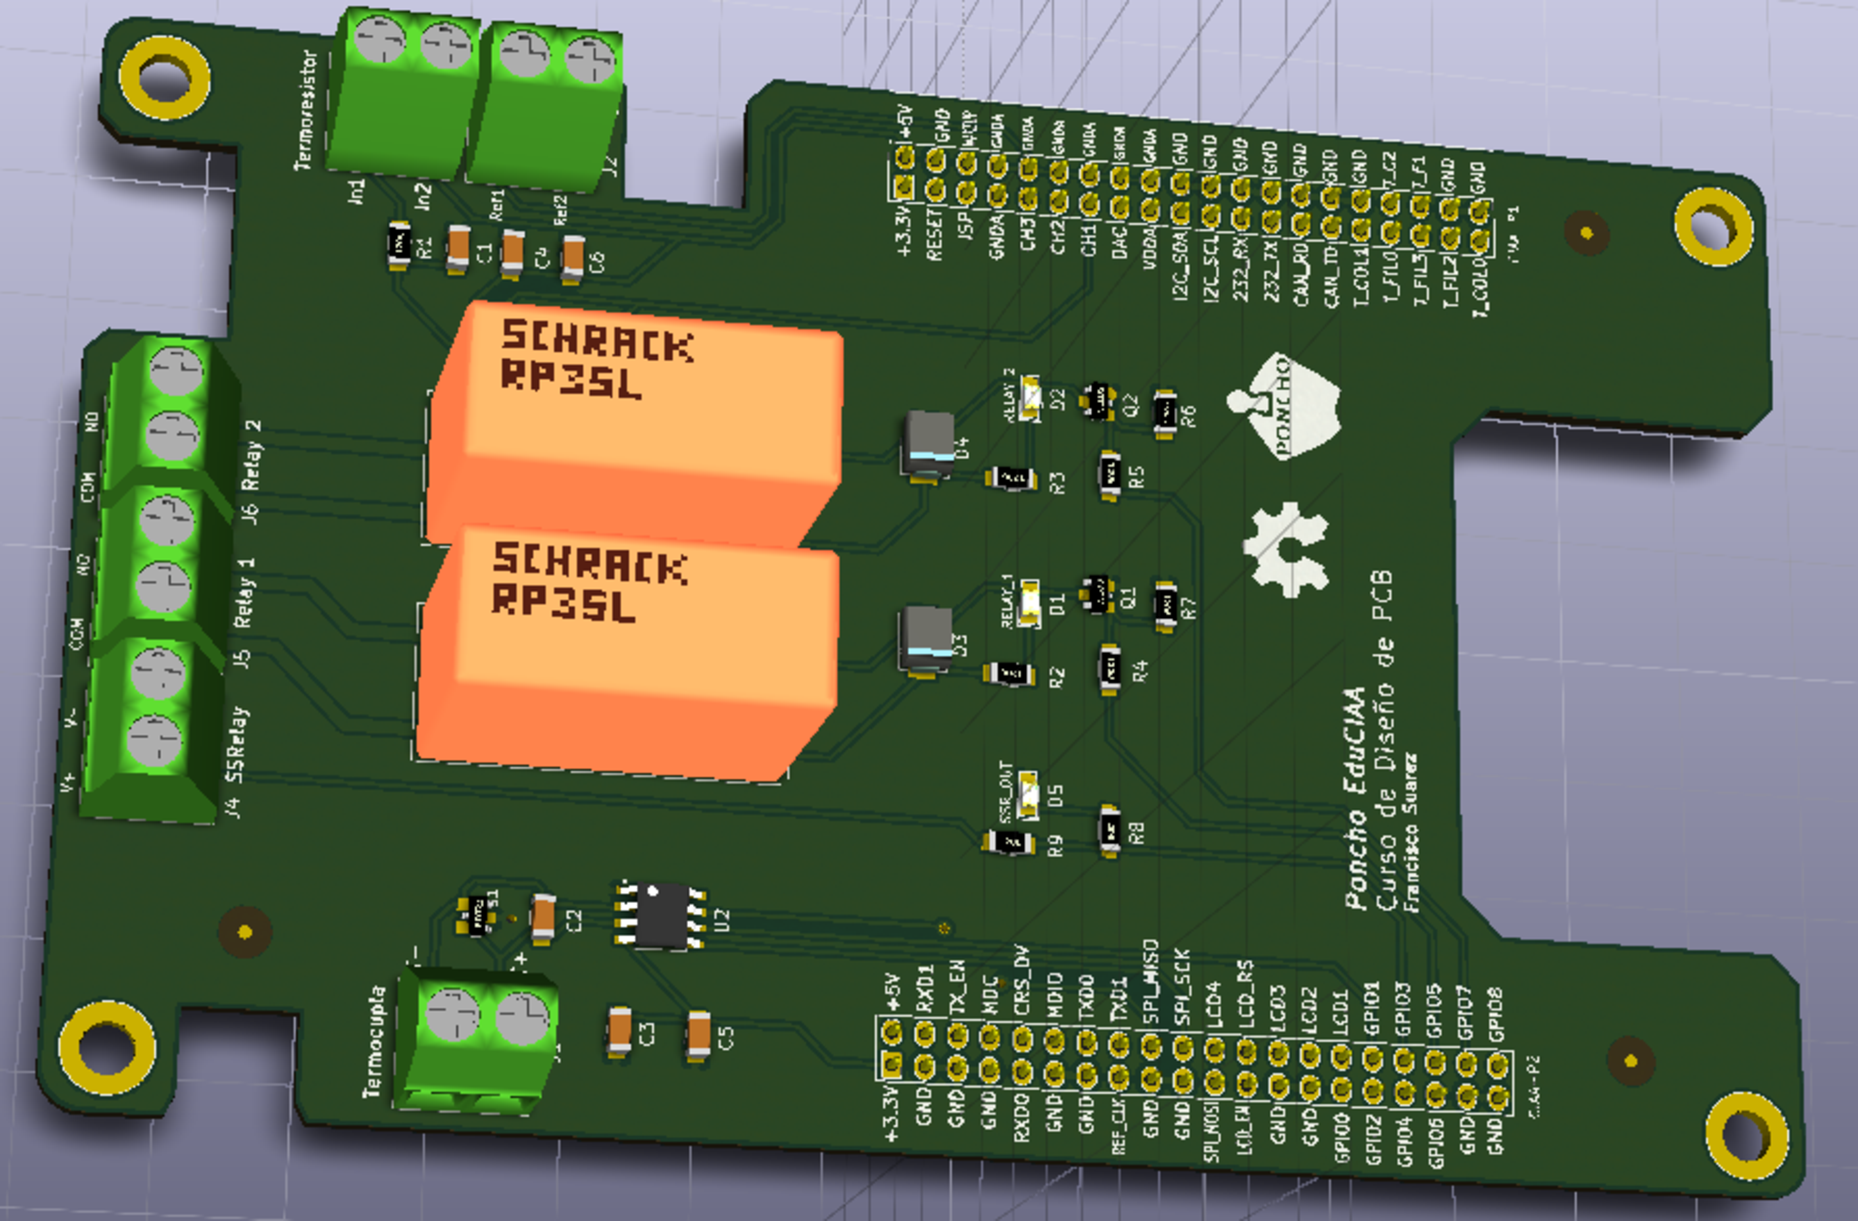
\includegraphics[width=.7\textwidth]{Figures/Cap_3/tempRelayPoncho_TOP}
	\caption{Render vista de arriba placa de interfaz.}
	\label{fig:renderPonchoTOP}
\end{figure}

\begin{figure}[h!]
	\centering
	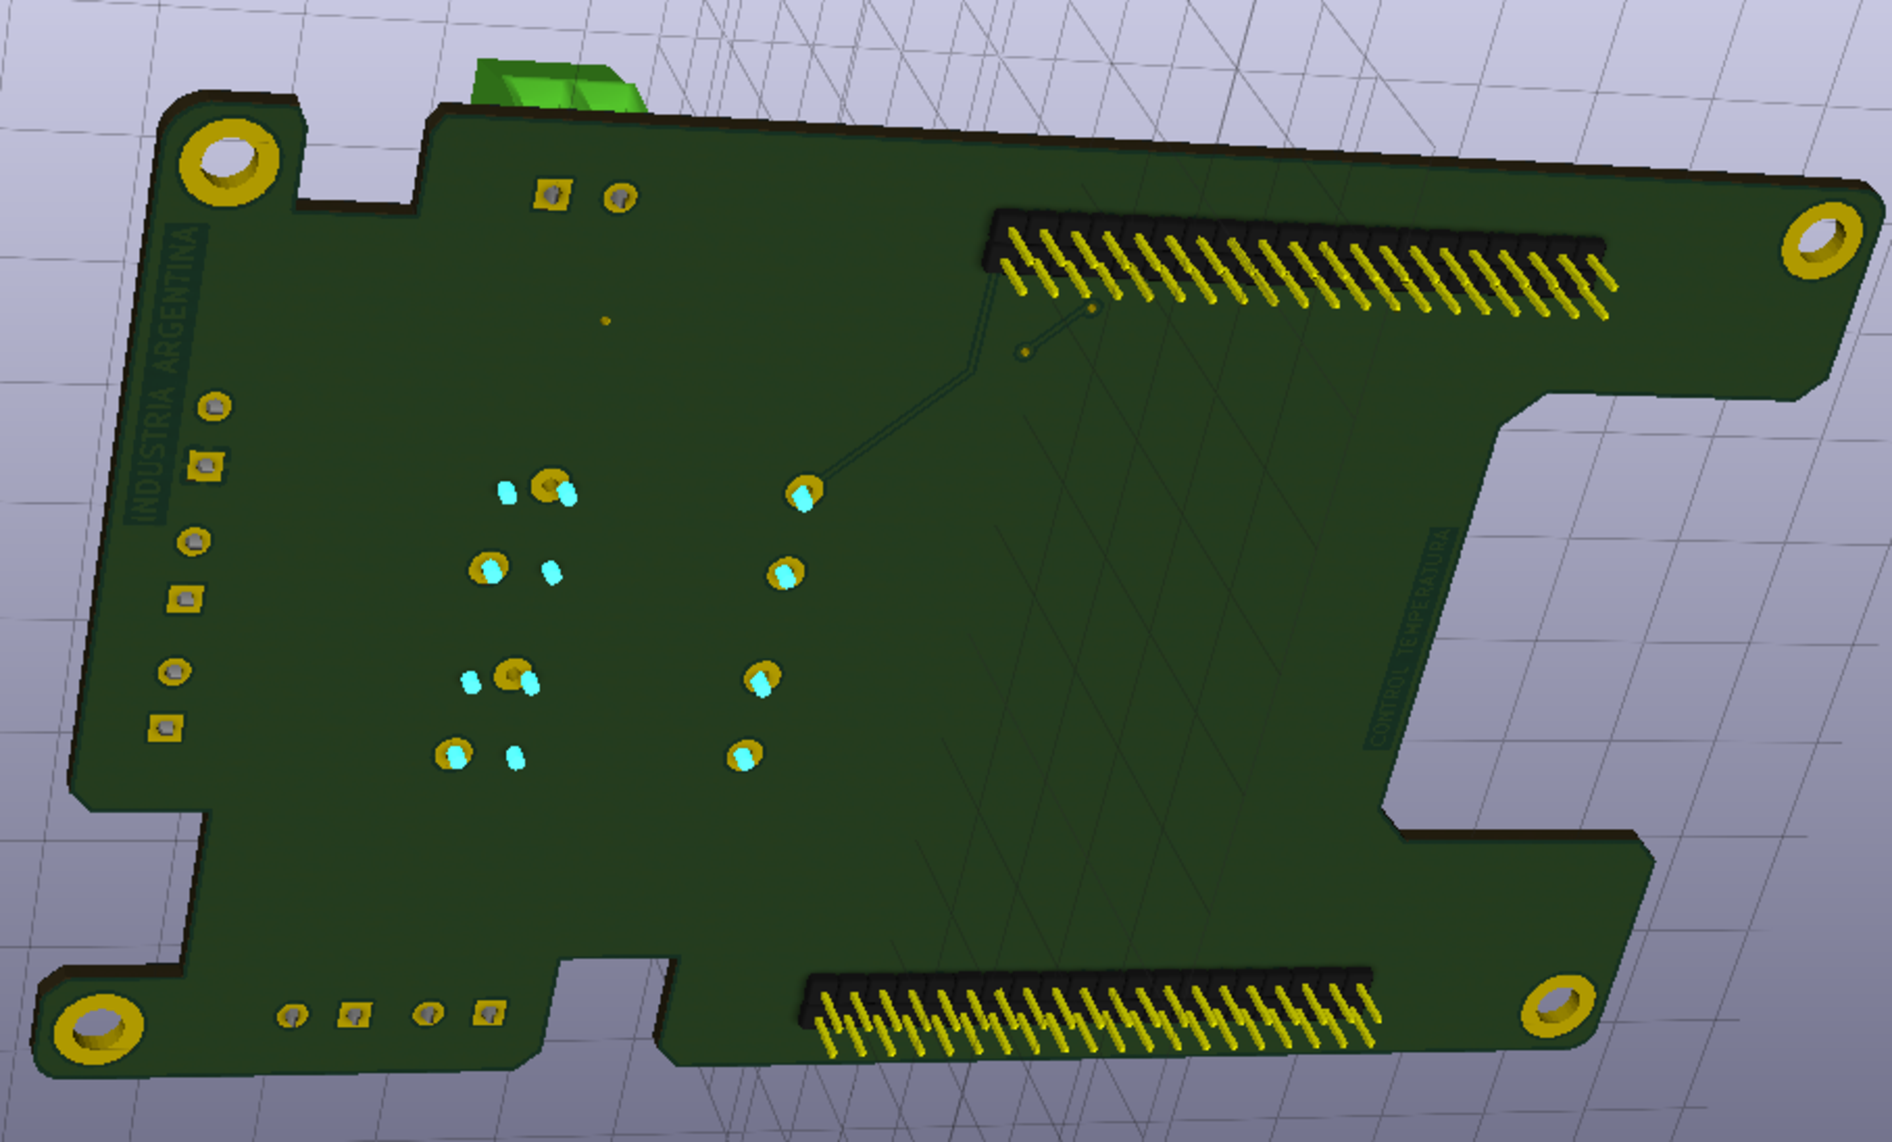
\includegraphics[width=.7\textwidth]{Figures/Cap_3/tempRelayPoncho_BOTTOM}
	\caption{Render vista de abajo de placa de interfaz.}
	\label{fig:renderPonchoBOT}
\end{figure}

La placa de la figura no llego a construirse hasta la fecha debido a que no se habían terminado de definir detalles relevantes respecto al numero y tipos de sensores y actuadores a utilizar.

En el Apéndice \ref{AppendixB} se encuentran los esquemáticos completos de las placa de expansión.
%----------------------------------------------------------------------------------------
%	SECTION 2
% La idea de esta sección es resaltar los problemas encontrados, los criterios utilizados y la justificación de las decisiones que se hayan tomado.
%----------------------------------------------------------------------------------------
\section{ Arquitectura del Software }

En función de los requerimientos vistos en \ref{subsec:Requerimientos} y de implementar los conocimientos aprendidos durante el posgrado, se determinaron los criterios para esta etapa.\\ 
En primer lugar se eligió usar lenguaje C y el sistema operativo FreeRTOS para la implementación.\
En segundo se diseñó el código de manera modularizado en tareas las cuales pueden funcionar de modo independiente según si la implementación lo requiere. \
En tercer lugar se tiene como modelo patrón el denominado \enquote{control ambiental} el cual se emplea cuando es un sistema con sensores que proporcionan información sobre el entorno y los actuadores pueden cambiar.\\

La aplicación cuenta los siguientes componentes:
\begin{itemize}
\item a.Interfaz de usuario (ingreso de parámetros, uart, lcd, alarmas).
\item b.Control de temperatura.
\item c.Monitoreo de nivel.
\item d.Monitoreo de conductividad.
\item e.Monitoreo de energía.
\item f.Control de tiempos.
\end{itemize}

Según el modo de funcionamiento seleccionado se tendrá una diferente configuración del software siempre dentro de la misma arquitectura y con pocas diferencias entre ellos. En la figura \ref{fig:diag_interfaces_m1} se muestran los diagramas de interfaces y procesos internos en el modo de funcionamiento 1. 
% AGREGAR UN DIAGRAMA DE INTERACCION ENTRE COMPONENTES ¿? ******************************
\begin{figure}[h!]
	\centering
	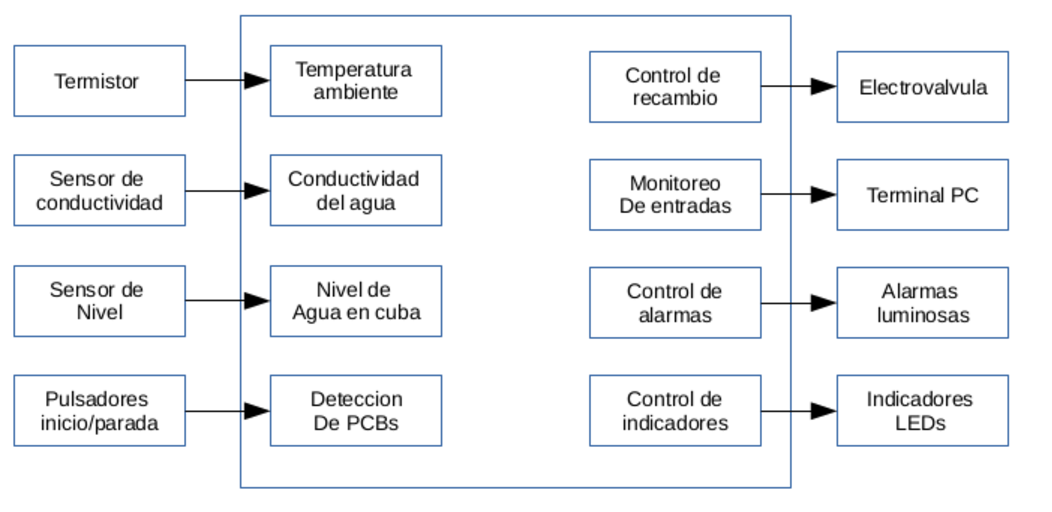
\includegraphics[width=1.0\textwidth]{Figures/Cap_3/diagrama_interfaces_1}
	\caption{ Vinculación de las periféricos del sistema con las interfaces internas en el modo 1. }
	\label{fig:diag_interfaces_m1}
\end{figure}
 
En la figura \ref{fig:diag_comunicacion_m1} se muestra el diagrama de comunicación entre los procesos originados para el caso de funcionamiento 1. Se nota su relación con los componentes de la aplicación: a,b,e y f.

\begin{figure}[h!]
	\centering
	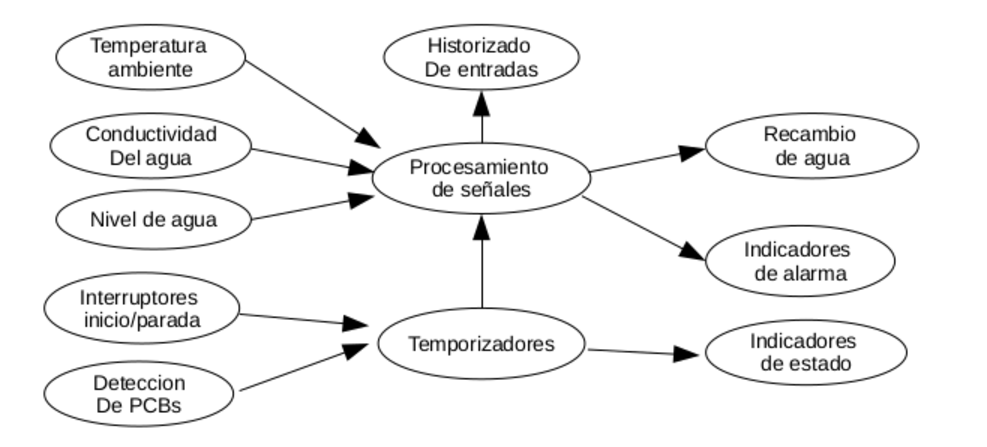
\includegraphics[width=1.0\textwidth]{Figures/Cap_3/diagrama_comunicacion_1}
	\caption{ Diagrama de comunicación entre procesos en el modo 1. }
	\label{fig:diag_comunicacion_m1}
\end{figure}
 
En la figura \ref{fig:diag_interfaces_m2} se muestran los diagramas de interfaces y procesos internos en el modo de funcionamiento 2.  Se nota que hay poca diferencia con el caso anterior, solo tienen activos otros procesos de interfaz.

\begin{figure}[h!]
	\centering
	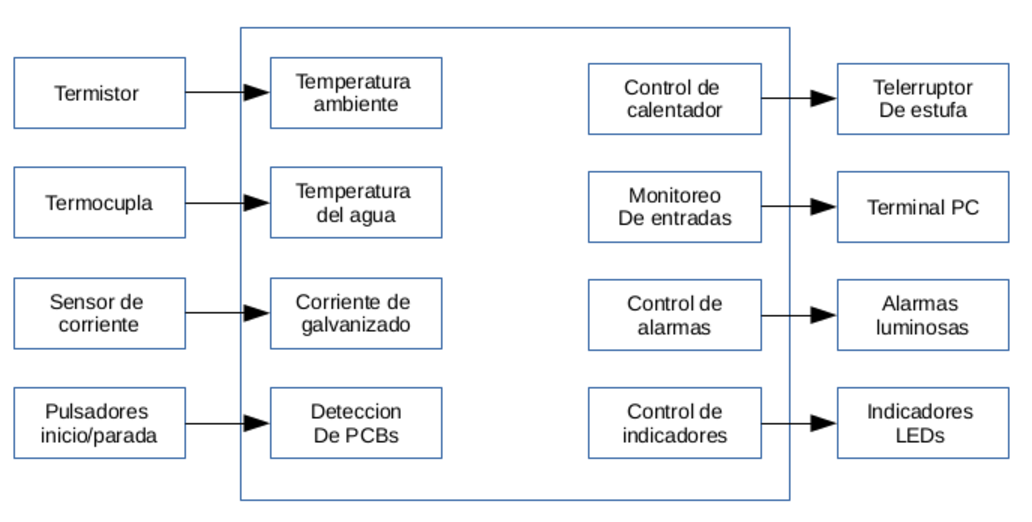
\includegraphics[width=1.0\textwidth]{Figures/Cap_3/diagrama_interfaces_2}
	\caption{ Vinculación de las periféricos del sistema con las interfaces internas en el modo 2.}
	\label{fig:diag_interfaces_m2}
\end{figure}

En la figura \ref{fig:diag_comunicacion_m2} se muestra el diagrama de comunicación entre los procesos originados para el caso de funcionamiento 2. Se nota su relación con los componentes de la aplicación: a,b,c, y f.

\begin{figure}[h!]
	\centering
	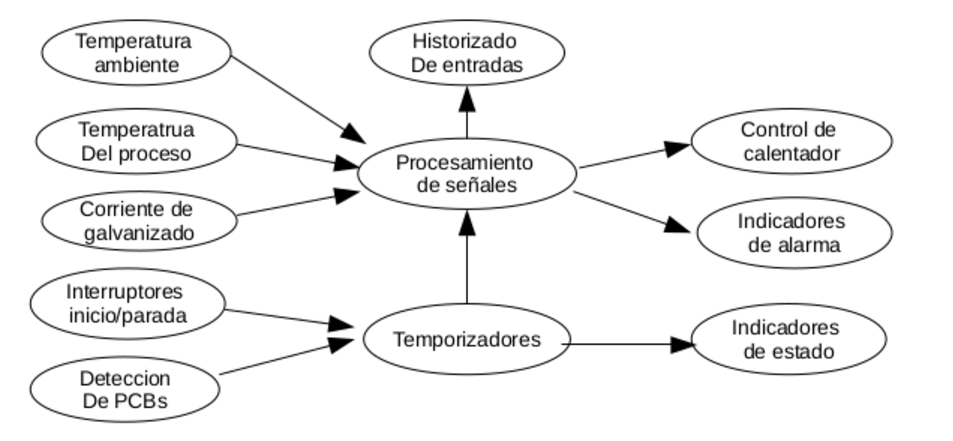
\includegraphics[width=1.0\textwidth]{Figures/Cap_3/diagrama_comunicacion_2}
	\caption{ Diagrama de comunicación entre procesos en el modo 2. }
	\label{fig:diag_comunicacion_m2}
\end{figure}
 
\subsection{ Capas de abstracción }

el sistema se divide en capas que otorgan abstracción del hardware y además permiten obtener código mas reutilizable e independiente de la plataforma. Estos son cambios que el cliente puede solicitar a futuro.
En la figura \ref{fig:diagrama_capas} se observa el patrón de capas de la arquitectura.

% Agregar una imagen con la division en capas del firmware.
\begin{figure}[h!]
	\centering
	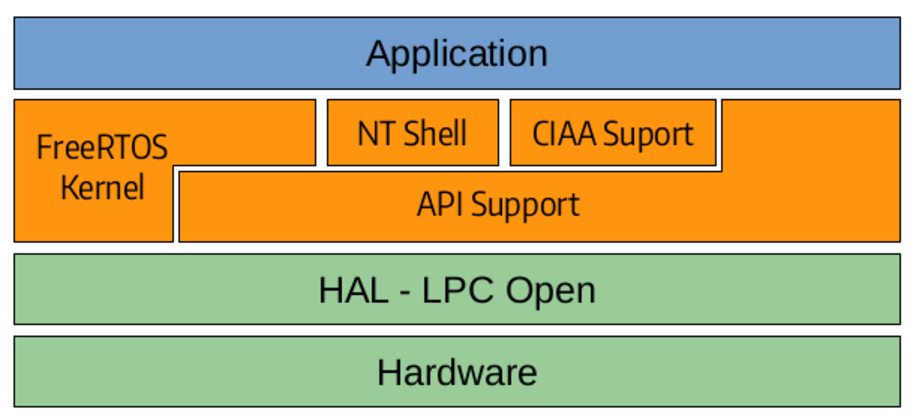
\includegraphics[width=.8\textwidth]{Figures/Cap_3/diagrama_capas}
	\caption{Estructuras de capas del sistema.}
	\label{fig:diagrama_capas}
\end{figure}
 
Las capas son las siguientes: 
\begin{itemize}
\item \emph{Aplicación:} Rutinas creadas para cada una de las tareas.
\item \emph{NT Shel:} Implementa el interprete de comandos ingresados externamente e internamente, a fin de configurar o de obtener información del dispositivo \citep{nt_shell}.
\item \emph{FreeRTOS:} Sistema operativo, controla la comunicación entre tareas, acceso a recursos compartidos y el scheduler. \cite{free_rtos}.
\item \emph{API Support:} implementa las rutinas de acceso y configuración de los distintos periféricos.
\item \emph{HAL:} rutinas de acceso al hardware, implementada con la librería LPC OPEN para el uP LPC43XX \citep{lpcopen}.
\end{itemize}


\subsection{ Diseño }

Por la necesidad de dividir el problema en partes menores para hacerlo mas escalable, mantenible y debugueable, el sistema se divide en subsistemas o tareas cooperativas entre si. Las mismas están definidas como:
\begin{itemize}
	\item Monitoreo de entradas analógicas-digitales.
	\item Control de salidas digitales.
	\item Manejo de terminal y comandos.
	\item Manejo de memoria y log de datos.
\end{itemize}

En la figura \ref{fig:diag_Tareas} muestra un diagrama de estado general de las tareas y la interacción entre ellas.
% Diagrama de tareas y conexion entre ellas
\begin{figure}[h!]
	\centering
	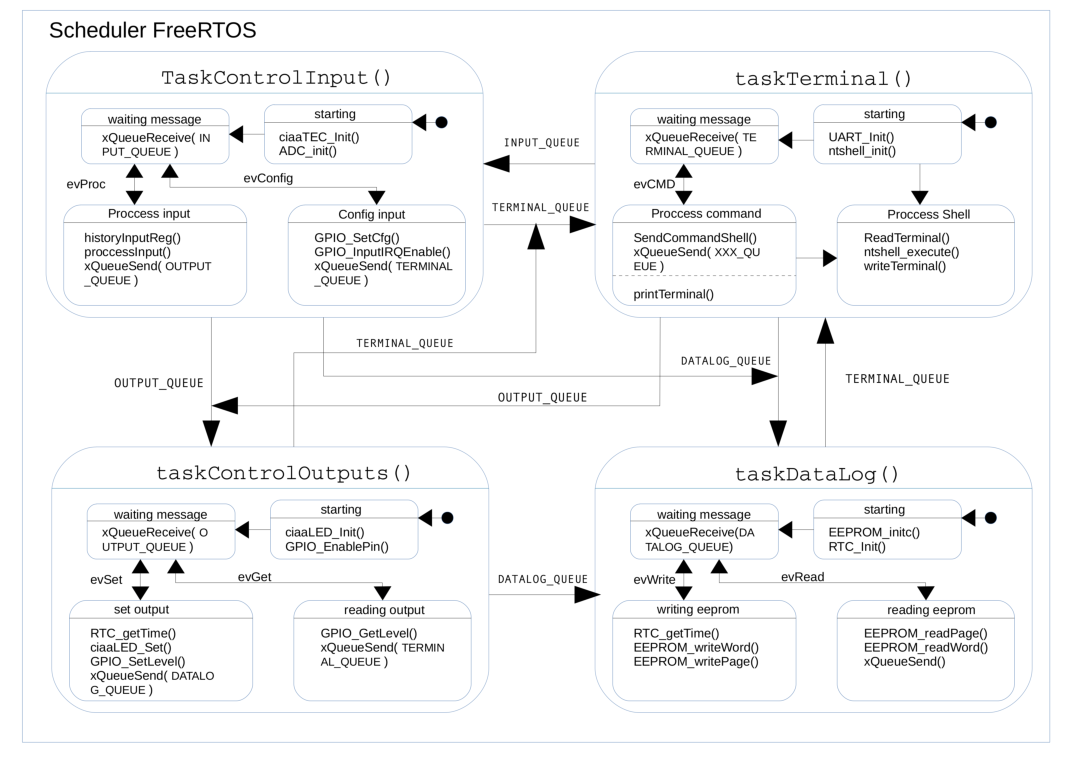
\includegraphics[width=1.2\textwidth]{Figures/Cap_3/diagrama_tareas}
	\caption{ Interacción entre tareas. }
	\label{fig:diag_Tareas}
\end{figure}

\section{ Sistemas control de entradas }
El monitoreo de las entradas se divide en subestados según la opción de funcionamiento elegida, y a la vez se puede encontrar en funcionamiento normal, en estado falla o en reconfiguración. 
La lectura de las entradas digitales las hace por interrupción mientras que las analógicas las hace por polling según tiempos por default a través del terminal. La figura \ref{fig:diag_TareasInp} muestra el diagrama de estados de la tarea.
 
% Se puede pensar tambien en poder poner la tarea en suspension hasta no tener una habilitacion por algun semaforo o por alguna tarea que la suspenda, tendria que ser si o si la taskTerminal. O bien por algun estado de error que la deje esperando la normalizacion. 
\begin{figure}[h!]
	\centering
	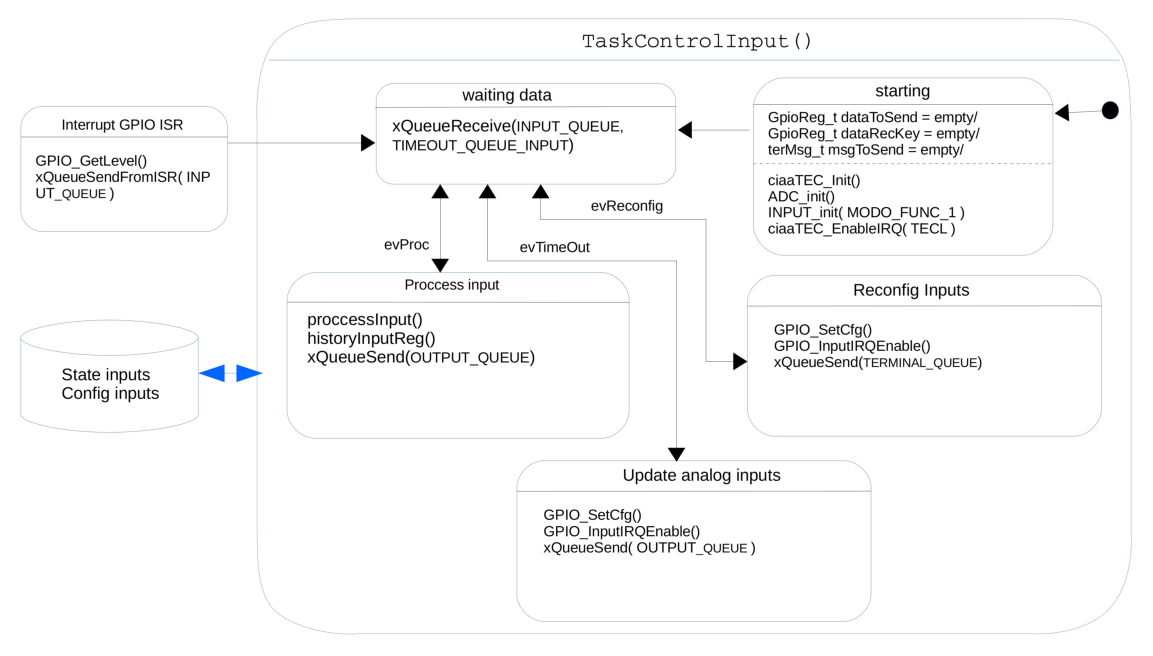
\includegraphics[width=1.2\textwidth]{Figures/Cap_3/diagrama_tarea_input}
	\caption{ Diagrama de estados de la tarea control de entradas. }
	\label{fig:diag_TareasInp}
\end{figure}

Se observa que a medida que se actualizan los valores de las registros de las entradas, la tarea ejecuta acciones vinculadas con cada una de ellas. Luego en función de estas acciones evalúa si debe enviar un mensaje hacia otra de las tareas, siempre y cuando la tarea destino esté habilitada y en modo activo.
El manejo de los temporizadores de duración de cada etapa es implementado por esta tarea, ya que es dependiente del estado de entradas digitales.   

\section{ Sistemas control de salidas }
El control de las salidas esta ligado expresamente a las acciones externas. Las acciones llegan por cambios ocurridos en las entradas o pueden ser forzar a través del terminal de PC. Por esta razón éste modulo no es pausado en ningún momento del funcionamiento.\\
Las acciones que activan las salidas están parametrizadas en un registro interno del módulo. Cuando la tarea verifica que se debe ejecutar un cambio en una salida entonces verifica también si debe reenviar algún parámetro hacia otra tarea.
La figura \ref{fig:diag_TareasOut} muestra el diagrama de estados de la tarea.
 
\begin{figure}[h!]
	\centering
	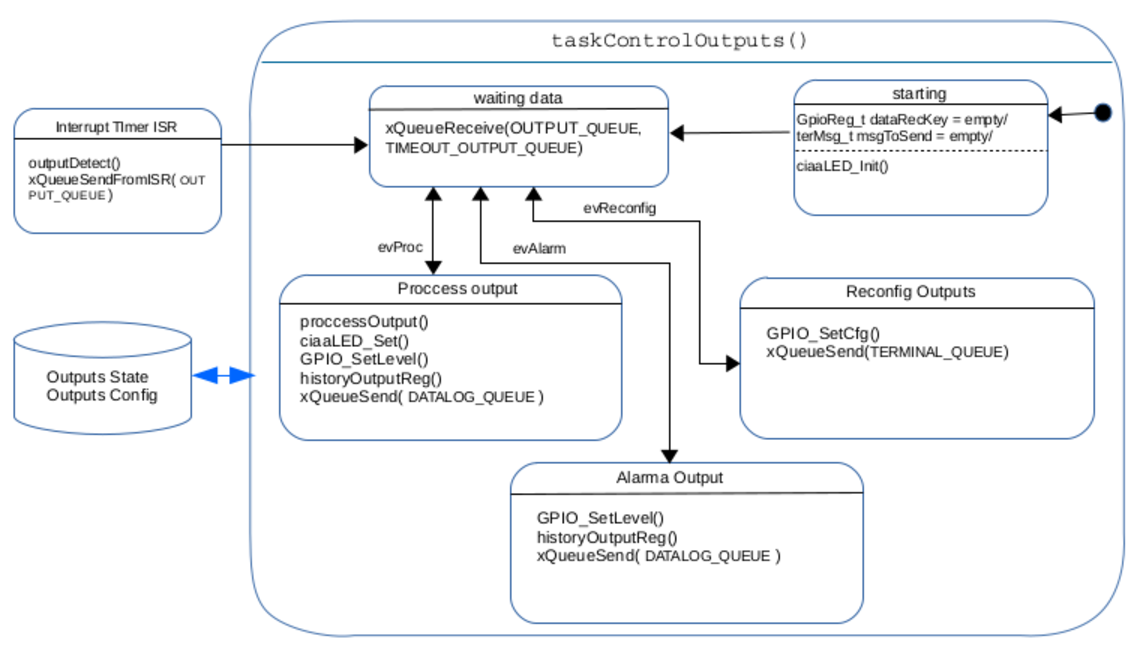
\includegraphics[width=1.2\textwidth]{Figures/Cap_3/diagrama_tarea_output}
	\caption{ Diagrama de estados de la tarea control de salidas. }
	\label{fig:diag_TareasOut}
\end{figure}

\section{ Sistemas control de terminal-Shell }
Este modulo se encarga de emular la terminar con la PC procesando comandos y consultas. Esta tarea es opcional para el sistema pero es importante para obtener información de históricos y realizar test de los puertos del hardware. 
%---- VER si queda este parrafo.
Originariamente se pensó también que la misma ajustaría los parámetros de alarma y de tiempos por etapa a partir del ingreso de información del lote a procesar. Luego como se determino que el sistema fueran modular este concepto no es aplicable. No obstante se pueden ajustar parámetros de tiempos y de niveles de alarma.

La figura \ref{fig:diag_TareasShell} muestra el diagrama de estados de la tarea.
% Colocar diagrama de estados
\begin{figure}[h!]
	\centering
	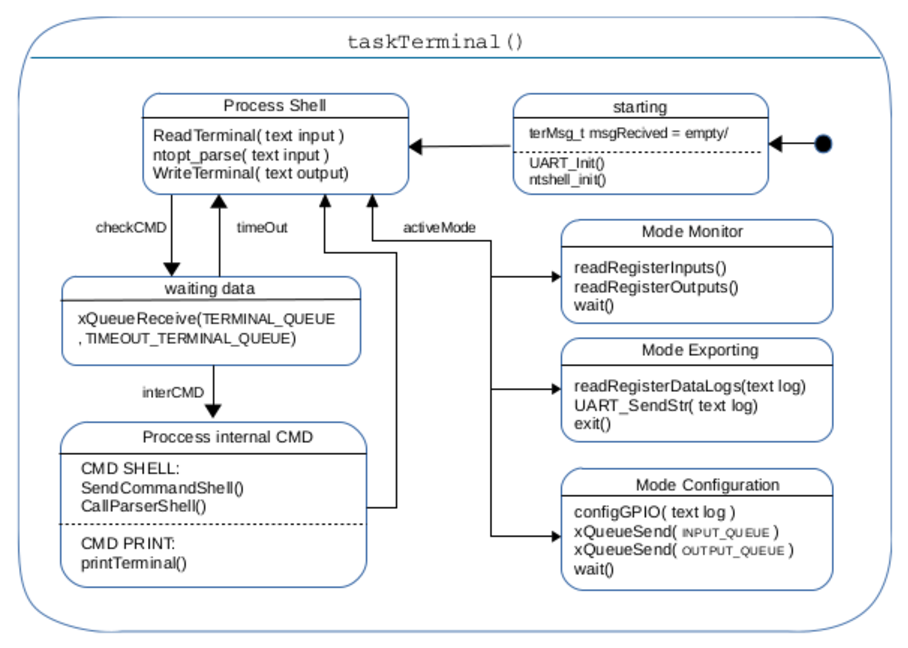
\includegraphics[width=1.2\textwidth]{Figures/Cap_3/diagrama_tarea_terminal}
	\caption{ Diagrama de estados de la tarea terminal de comunicación. }
	\label{fig:diag_TareasShell}
\end{figure}

Los estados están predeterminados por los comandos implementados de los cuales se puede agregar hasta 255. En la tabla \ref{tablas_comandos} se resumen los comandos implementados.

\begin{table}[h!]
\begin{flushleft}
\begin{tabular}{|m{1.5cm}|m{3cm}|m{4.2cm}|m{4.2cm}|}\hline
{\textbf{Comando}} & {\textbf{Función}} & {\textbf{Descripción}} & {\textbf{Parámetros}} \\ \hline
{\textit{hist}} & {Registros históricos} & { devuelve una lista de parámetros en formato csv (coma separated value) con los últimos registros guardados en memoria.} & {Ninguno} \\ \hline
{\textit{mon}} & {monitoreo de puertos} & {muestra en pantalla el valor y la variación de las entradas y salidas del dispositivo en función del modo de funcionamiento.} & {Ninguno.} \\ \hline
{\textit{conf}} & {Configuración de parámetros} & {Configura pines asignados, valores de alarma, tiempos de muestreo.} & {nXmax, nXmin, tXmax, tXmin. X: Número de parámetro. n: Nivel. t: Tiempo.} \\ \hline
{\textit{test}} & {testing de puertos} & {permite modificar el valor de los salidas o de una entrada para evaluar el comportamiento del sistema.} & {PX val, donde P=I/O, X=id puerto, val= valor del puerto..} \\ \hline
{\textit{time}} & {monitoreo de puertos} & {permite modificar la hora y fecha del calendario interno usado en la grabación de históricos.} & {c DDMMAA, calendario día(DD), mes(MM), año(AA).t HHMMSS, tiempo hora(HH), minutos(MM), segundos(SS).} \\ \hline
\end{tabular}
\end{flushleft}
\caption{Descripción tablas de comandos.}
\label{tablas_comandos}
\end{table}


\section{ Sistemas gestión de datos }

Se encarga de manejar los registros que deben ser guardados y leídos de la memoria EEPROM interna. Los datos a ser grabados son leídos de espacios de memoria RAM compartidos y los datos leídos son almacenados en un buffer compartido de la tarea para luego ser enviados a la tarea solicitante.
% Colocar diagrama de estados
La figura \ref{fig:diag_TareasLogs} muestra el diagrama de estados de la tarea.

\begin{figure}[h!]
	\raggedleft
	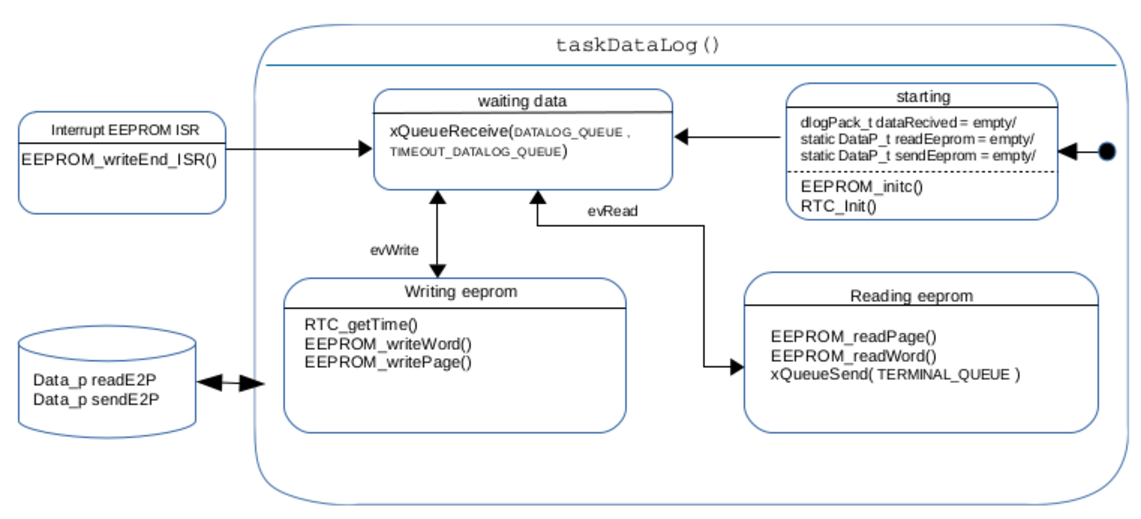
\includegraphics[width=1.2\textwidth]{Figures/Cap_3/diagrama_tarea_datalog}
	\caption{Diagrama de estados de la tarea manejo de datos en memoria.}
	\label{fig:diag_TareasLogs}
\end{figure}





